\documentclass[10pt,conference,compsocconf]{IEEEtran}

%\usepackage{times}
%\usepackage{balance}
\usepackage{url}
\usepackage{graphicx}	% For figure environment
\usepackage{url}
\usepackage{multirow}
\usepackage{array}
\graphicspath{ {./media/} }

\begin{document}
\title{Road Segmentation from Aerial Images}

\author{
\begin{tabular}{*{3}{>{\centering}p{5.5cm}}}
\large Francesco Saverio Varini & \large Robin Bader & \large Jakob Beckmann \tabularnewline
Department of Computer Science, & Department of Computer Science, & Department of Computer Science, \tabularnewline
ETH Zurich & ETH Zurich & ETH Zurich
\end{tabular}
}


\maketitle

\begin{abstract}
  This project deals with semantic segmentation of aerial images where a semantic labeling of road or non-road is assigned to patches on the images. Recently, \textit{deep convolutional neural networks} (CNNs) have shown impressive performance. Our method uses an adapted version of the U-Net \cite{Ronneberger2015} architecture which enables us to predict the full pixel images to patches and additionally propose to use augmentation and dropout layers to overcome the sparsity of the available training data. Our experiments show, that this model outperforms the other tested techniques.
\end{abstract}

\section{Introduction}

Understanding an image and extracting its information is an important area of application in computer vision. Image segmentation is the process of labeling parts of images according to given criteria. This paper focuses on the automatic segmentation of aerial images into \textit{road} or \textit{non-road} which has several application due to numerous real-world applications ranging from civil infrastructure~\cite{Radopoulou2016} to updating geographical information systems~\cite{Girres2010}.

The most popular tool for that task is supervised machine learning and the recent increase in computing resources has led to the development of new techniques such as \textit{deep convolutional neural networks} (CNN) which are currently top-performers for image segmentation. They have found broad attention in previous research of road segmentation~\cite{Kaiser2017,Saito2015}, but focused on a prediction of per-pixel segmentations or multiple-class segmentation. This project focuses on the prediction of patches in the images with exactly two classes.

We adopted the \textit{U-Net}~\cite{Ronneberger2015} architecture which is a variant of the \textit{Fully Convolution Network} (FCN)~\cite{Long2014} which predicts pixel-to-pixel segmentations. Our contribution is an adapted architecture of the U-Net which allows a pixel-to-patch segmentation and uses a different activation function as well as a dropout layer to prevent overfitting while overcoming the sparsity of the data with image augmentation.

We compare our approach to different baseline algorithms, specifically the standard U-Net implementation and the proposed patch-to-patch approach presented in \cite{Pavllo2017}.

\section{Models and Methods}

The contribution of this paper is a CNN architecture that takes as input an image and outputs the prediction of image-patches whether a certain area, given a threshold of 25\%, of each patch contains roads. This section describes the given datasets, which pre-processing techniques used, the proposed model’s architecture and the baseline which we compare our method to.

\subsection{Dataset \& Preprocessing}

The dataset is provided by the Kaggle competition during the ETH Computational Intelligence Lab 2018 \cite{KaggleCompetition} and contains 100 training samples that consists of an input image and its pixelwise labeling with a resolution of 400x400 pixels. The competition’s goal is to predict 16x16 sized patches within an input image of resolution 608x608 where every patch is labeled as 1 if more than 25\% of the patch’s area is labeled as road and labeled 0 otherwise.

The training dataset is preprocessed due to the fact that it is of different dimensions than the target images. Figure \ref{fig:preprocessing} visualizes the implemented preprocessing where the images are extended using a mirror boundary condition, i.e. the image is reflected along the boundary axis (See Figure \ref{fig:preprocessing}, right).

\begin{figure}
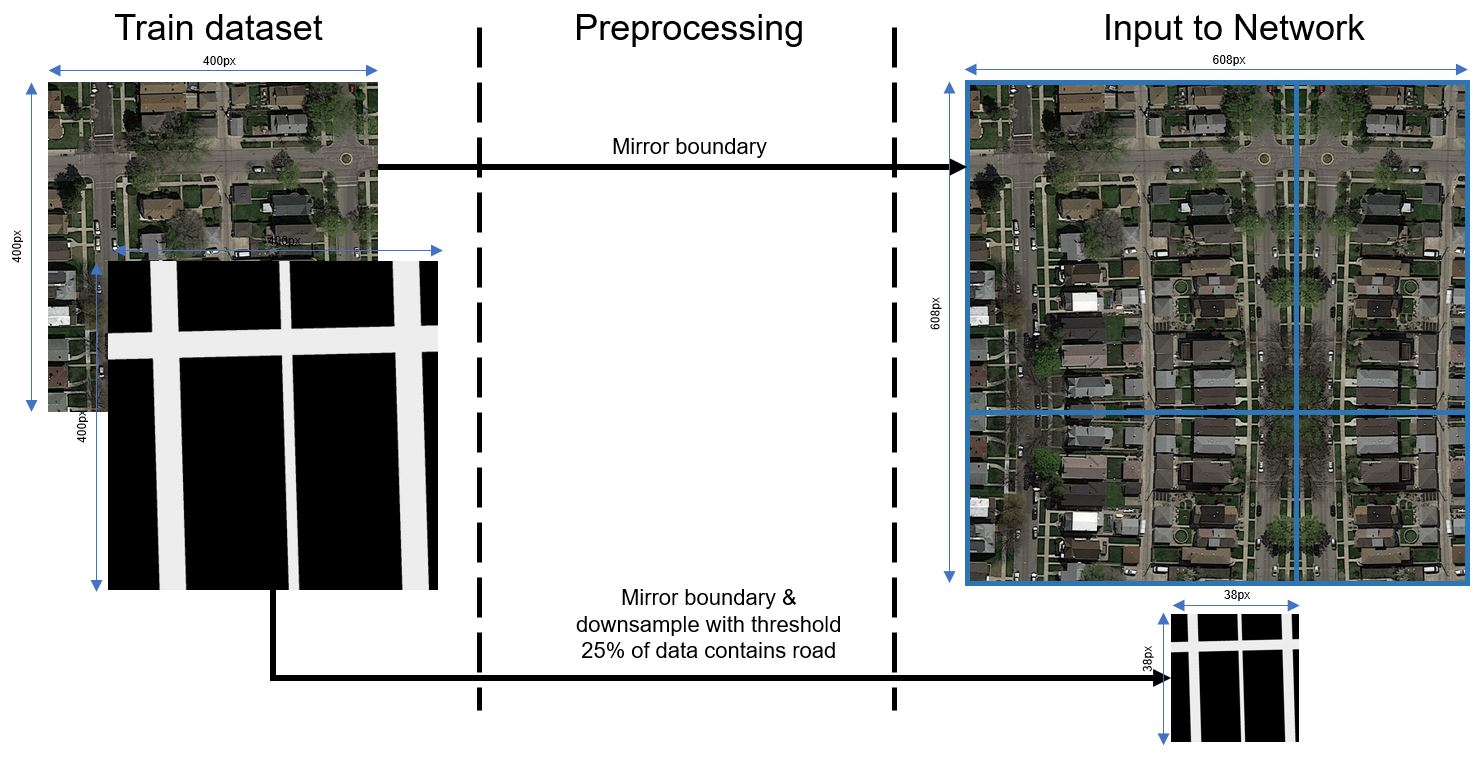
\includegraphics[width={8cm}]{preprocessing}
\caption{Preprocessing necessary for the training data. The given dataset (left) with dimensions 400x400 and its pixelwise labeling is preprocessed (middle) using a mirror effect which enlarges the images to a resolution of 608x608 (right). Furthermore, the labels are downsampled to a 38x38 for each 16x16 image patch.}
\label{fig:preprocessing}
\end{figure}

\subsection{Image Augmentation}

To overcome the limitation of the small training set we use data augmentation. The effectiveness of data augmentation was previously demonstrated \cite{Wang} for image classification. Because the roads of many of the provided training samples are axis aligned we decided to implement data augmentation that arbitrarily rotates the images compared to previous approaches with multiples of 90 degree \cite{Pavllo2017}. The disadvantage of our approach is that the generation of arbitrary rotations takes considerably more time. To maintain the advantage of the U-Net architecture of its fast training time \cite{Ronneberger2015} the augmentation steps are split into two groups which differ from its execution time. The first group is only executed once for every epoch while the latter is applied to each training sample for each batch.

The first group of augmentation steps applies randomly a zooming (range 0.8-1.2), shearing (range 0 - 0.1), rotation (0 – 360) and height as well as width shifting (range 0 - 0.1). Finally, before generating each batch as input to the model we apply additional a multiple of a 90-degree rotation as well as a random mirroring. This second step can be executed very fast during training time while the first step needs more time. This technique enabled us to overcome the disadvantage of slow arbitrary rotation while still generating a high number of different training samples.

\subsection{CNN Architecture}

\begin{figure}
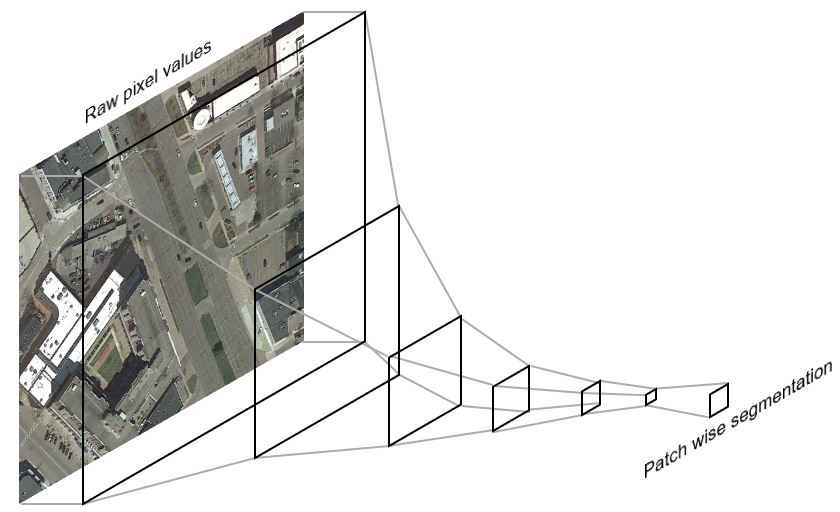
\includegraphics[width={8cm}]{network-visualisation}
\caption{Architecture of the proposed network. Visualizing the 7 layers used where the first 6 downsample the image and the 7th layer upsamples it again using a residual connection to layer 5 and outputs a patch wise segmentation.}
\label{fig:architecture}
\end{figure}

To achieve the desired pixel-to-patch prediction of the model we adapted a truncated version of the U-Net \cite{Ronneberger2015} as presented in Table \ref{table:truncated_unet} which is further visualized in Figure \ref{fig:architecture}. The original implementation of the U-Net uses the up-sampling layer (e.g. layer 7) as many times as the down-sampling layers (e.g. layer 1 – 4) to output the same dimensions as the input. In this project this isn't desired, and the model has been truncated to fit our needs where the dimension 38x38 corresponds to the desired path size $16 \cdot 38 = 608$.

To further accommodate arising overfitting of the training data a further adapted version with regularization is proposed as shown in Table \ref{table:truncated_regularized_unet}. These adaptions where influenced by \cite{Pavllo2017}. Instead of using \textit{rectified linear units} (ReLU) as activation function as proposed by the U-Net implementation \cite{Ronneberger2015} we replace them with \textit{Leaky ReLUs} to avoid the \textit{dead filter effect} which some units can experience. \textit{Leaky ReLUs} are defined as $f(x) = \max(\alpha x, x)$ where we found by experimentation the value $\alpha=0.1$ yields good results as found in other methods \cite{Pavllo2017}. Furthermore, to regularize the model we added after each level a dropout layer with a dropout rate of $0.25$. The output layer is further controlled using a L2-regularizer.

\begin{table}[]
\centering
\begin{tabular}{lll}
\hline
Level & Layer                                                                       & Dimension  \\ \hline
0     & input                                                                       & 608x608x3  \\
1     & \begin{tabular}[c]{@{}l@{}}2 x conv(3x3, ReLU)\\ maxpool(2x2)\end{tabular}  & 304x304x32 \\
2     & \begin{tabular}[c]{@{}l@{}}2 x conv(3x3, ReLU)\\ maxpool(2x2)\end{tabular}  & 152x152x64 \\
3     & \begin{tabular}[c]{@{}l@{}}2 x conv(3x3, ReLU)\\ maxpool(2x2)\end{tabular}  & 76x76x128  \\
4     & \begin{tabular}[c]{@{}l@{}}2 x conv(3x3, ReLU)\\ maxpool(2x2)\end{tabular}  & 38x38x256  \\
5     & 2 x conv(3x3, ReLU)                                                         & 19x19x512  \\
6     & \begin{tabular}[c]{@{}l@{}}up-conv(2, 2)\\ 2 x conv(3x3, ReLU)\end{tabular} & 38x38x256  \\
7     & conv(1x1, Sigmoid)                                                          & 38x38x1    \\ \hline
\end{tabular}
\caption{U-Net, truncated for pixel to patch prediction.}
\label{table:truncated_unet}
\end{table}

\begin{table}[]
\centering
\begin{tabular}{lll}
\hline
Level & Layer                                                                       & Dimension  \\ \hline
0     & input                                                                       & 608x608x3  \\
1     & \begin{tabular}[c]{@{}l@{}}2 x conv(3x3, Leaky ReLU)\\ maxpool(2x2) \\ dropout(0.25) \end{tabular}  & 304x304x32 \\
2     & \begin{tabular}[c]{@{}l@{}}2 x conv(3x3, Leaky ReLU)\\ maxpool(2x2) \\ dropout(0.25) \end{tabular}  & 152x152x64 \\
3     & \begin{tabular}[c]{@{}l@{}}2 x conv(3x3, Leaky ReLU)\\ maxpool(2x2) \\ dropout(0.25) \end{tabular}  & 76x76x128  \\
4     & \begin{tabular}[c]{@{}l@{}}2 x conv(3x3, Leaky ReLU)\\ maxpool(2x2) \\ dropout(0.25) \end{tabular}  & 38x38x256  \\
5     & \begin{tabular}[c]{@{}l@{}}2 x conv(3x3, Leaky ReLU)  \\ dropout(0.25)               \end{tabular}  & 19x19x512  \\
6     & \begin{tabular}[c]{@{}l@{}}up-conv(2, 2)\\ 2 x conv(3x3, Leaky ReLU)                 \end{tabular}  & 38x38x256  \\
7     & \begin{tabular}[c]{@{}l@{}}conv(1x1, Sigmoid)\\ L2(10E-6)                                 \end{tabular}  & 38x38x1    \\ \hline
\end{tabular}
\caption{U-Net, truncated, dropout \& LeakyRelu for pixel to patch prediction.}
\label{table:truncated_regularized_unet}
\end{table}

\subsection{Loss function}

The final score on the Kaggle competition \cite{KaggleCompetition} is calculated using the F1-Score which was used for the training the model as well.

\section{Results}

We evaluate our proposed model using a train/validation split of 2/3 of the dataset. The final 


\section{Discussion}

\section{Summary}


\bibliographystyle{IEEEtran}
\bibliography{bibliography}
\end{document}
